\section{Welche Konsistenzbeziehungen bestehen zwischen BPMN- und BROS-Modellen?}

\begin{frame}{Konsistenzproblem}
  Eine \textbf{Inkonsistenz} tritt genau dann auf, wenn eine Konsistenzregel verletzt wird.

  Eine \textbf{Konsistenzregel} ist eine Formalisierung von einem Aspekt der Konsistenz zwischen den betrachteten Modellen.

  Das \textbf{Konsistenzproblem} beschreibt den Vorgang der Minimierung und Verhinderung von Inkonsistenzen mit Hilfe der Aufstellung und Prüfung von Konsistenzregeln.

  TODO: Referenzen, Konsistenz
\end{frame}

\begin{frame}{Business Process Model and Notation}
  \begin{figure}
    \centering
    \begin{adjustbox}{width=1.1\linewidth,center}
      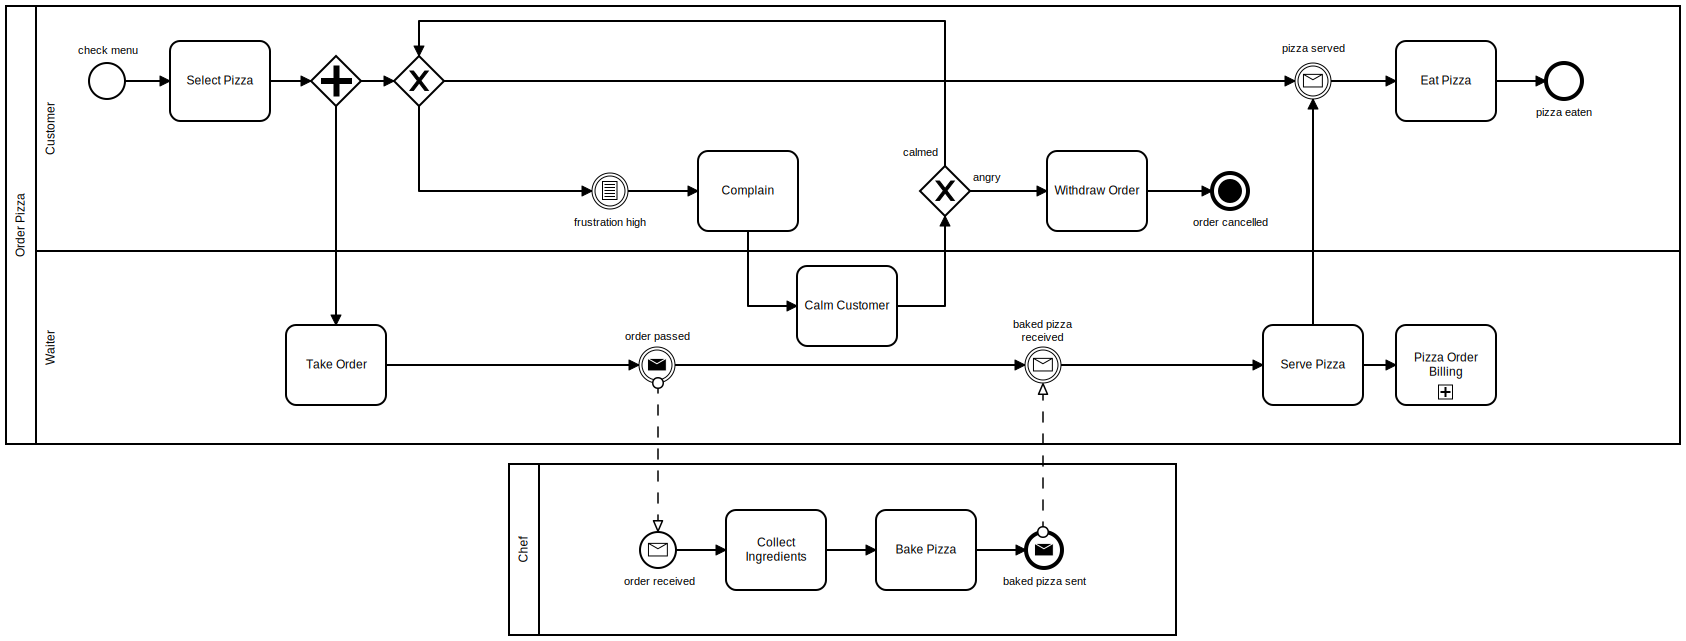
\includegraphics{images/example/bpmn.pdf}
    \end{adjustbox}
  \end{figure}
\end{frame}
\begin{frame}{Business Role-Object Specification}
  \begin{figure}
    \centering
    \begin{adjustbox}{width=0.9\linewidth,center}
      \includegraphics{images/example/bros-rule6.png}
    \end{adjustbox}
  \end{figure}
\end{frame}

\begin{frame}[fragile]{Prolog-Datenstrukutr}
\begin{lstlisting}[language=Prolog]
% Definition aller BPMN Elemente.
bpmn(Bpmn, Type).

% Definition aller BROS Elemente.
bros(Bros, Type).

% Definition aller Relationen.
relation(Source, Target, Type).

% Definition der Eltern-Kind Beziehung.
parent(Child, Parent).
\end{lstlisting}
\end{frame}
\begin{frame}[fragile]{Hilfsfunktionen}
\begin{lstlisting}[language=Prolog]
% Konsistenz der Eltern-Kind Beziehung.
check_parent(C) :- 
  parent(C, P), parent(C, Q) -> P == Q.

% Transitiver Abschluss der Modellstruktur.
transitive_parent(Child, Parent).

% Orakel für das Matching von Modellelementen.
match(Bpmn, Bros).
\end{lstlisting}
\end{frame}

\begin{frame}{Konsistenzbeziehungen}
  \begin{figure}
    \centering
    \begin{subfigure}{0.3\textwidth}
        \centering
        \begin{adjustbox}{width=0.8\linewidth,center}
          \begin{tikzpicture}
            \node at (0,0) {\begin{tikzpicture}[scale=0.5, every node/.style={scale=0.8},>={Latex[length=1.5mm]}]
  \draw[dashed] (-8,-7) -- (8,7);
  \draw (-6,-5.25) node[anchor=south, rotate=41] {\textbf{BPMN}};
  \draw (-6,-5.25) node[anchor=north, rotate=41] {BROS};

  \draw (-8,6) rectangle (0,1);
  \draw (-7,6) -- (-7,1);
  \draw (-7.5,3.5) node[rotate=90] {Order Pizza};
  \draw (-7,3.5) -- (0,3.5);
  \draw (-6.5,4.75) node[color=unimportant,rotate=90] {A};
  \draw (-6.5,2.25) node[color=unimportant,rotate=90] {B};

  \draw[rounded corners=4.8pt] (0,-0.5) rectangle (8,-6.5);
  \draw (0.2,-0.56) -- (0.2,-6.44);
  \draw (0,-1.5) -- (8,-1.5);
  \draw (4,-1) node {OrderPizza};

  \begin{scope}[color=unimportant]
      \draw[rounded corners=4.8pt] (4.2,-2) rectangle (7.2,-4);
      \draw (4.2,-3) -- (7.2,-3);
      \draw (4.2,-3.5) -- (7.2,-3.5);
      \draw (5.6,-2.5) node {A};

      \draw[rounded corners=4.8pt] (0.8,-4) rectangle (3.8,-6);
      \draw (0.8,-5) -- (3.8,-5);
      \draw (0.8,-5.5) -- (3.8,-5.5);
      \draw (2.4,-4.5) node {B};
  \end{scope}
\end{tikzpicture}
};
            \filldraw[draw=background,fill=background,fill opacity=0, draw opacity=0] (-4,-3.5) rectangle (4,3.5);
          \end{tikzpicture}
        \end{adjustbox}
        \caption*{\tiny{Regel 1: BPMN-Process}}%
    \end{subfigure}
    \hfill
    \begin{subfigure}{0.3\textwidth}
        \centering
        \begin{adjustbox}{width=0.8\linewidth,center}
          \begin{tikzpicture}
            \node at (0,0) {\begin{tikzpicture}[scale=0.5, every node/.style={scale=0.8},>={Latex[length=1.5mm]}]
  \draw[dashed] (-8,-7) -- (8,7);
  \draw (-6,-5.25) node[anchor=south, rotate=41] {\textbf{BPMN}};
  \draw (-6,-5.25) node[anchor=north, rotate=41] {BROS};

  \draw (-8,6) rectangle (0,1);
  \draw (-7,6) -- (-7,1);
  \draw (-7.5,3.5) node[rotate=90] {Chef};

  \draw[rounded corners=4.8pt,color=unimportant] (0,-0.5) rectangle (8,-6.5);
  \draw[color=unimportant] (0.2,-0.56) -- (0.2,-6.44);
  \draw[color=unimportant] (0,-1.5) -- (8,-1.5);
  \draw[color=unimportant] (4,-1) node {OrderPizza};

  \draw[rounded corners=4.8pt] (2.5,-3) rectangle (5.5,-5);
  \draw (2.5,-4) -- (5.5,-4);
  \draw (2.5,-4.5) -- (5.5,-4.5);
  \draw (4,-3.5) node {Chef};
\end{tikzpicture}
};
            \filldraw[draw=background,fill=background,fill opacity=0, draw opacity=0] (-4,-3.5) rectangle (4,3.5);
          \end{tikzpicture}
        \end{adjustbox}
        \caption*{\tiny{Regel 2: BPMN-Swimlane}}%
    \end{subfigure}
    \hfill
    \begin{subfigure}{0.3\textwidth}
        \centering
        \begin{adjustbox}{width=0.8\linewidth,center}
          \begin{tikzpicture}
            \node at (0,0) {\begin{tikzpicture}[scale=0.5, every node/.style={scale=0.8},>={Latex[length=1.5mm]}]
  \draw[dashed] (-8,-7) -- (8,7);
  \draw (-6,-5.25) node[anchor=south, rotate=41] {\textbf{BPMN}};
  \draw (-6,-5.25) node[anchor=north, rotate=41] {BROS};

  \draw (-8,6) rectangle (0,1);
  \draw (-7,6) -- (-7,1);
  \draw (-7.5,3.5) node[rotate=90] {Order Pizza};
  \draw (-6.5,4.5) node[rotate=90] {A};
  \draw (-6.5,2) node[rotate=90] {B};
  \draw (-7,3) -- (0,3);

  \begin{scope}[color=unimportant]
      \draw (-5,4.5) circle[radius=0.5];
      \draw (-5,4) node[anchor=north] {Start};
      \draw[->] (-4.5,4.5) -- (-2,4.5);
  \end{scope}
  \fill (-1.5,4.5) circle[radius=0.5];
  \fill[color=background] (-1.5,4.5) circle[radius=0.35];
  \fill (-1.5,4.5) circle[radius=0.2];
  \draw (-1.5,4) node[anchor=north] {End};

  \draw[rounded corners=4.8pt] (0,-0.5) rectangle (8,-6.5);
  \draw (0.2,-0.56) -- (0.2,-6.44);
  \draw (0,-1.5) -- (8,-1.5);
  \draw (4,-1) node {OrderPizza};

  \begin{scope}[color=unimportant]
      \draw[rounded corners=4.8pt] (4.2,-2) rectangle (7.2,-4);
      \draw (4.2,-3) -- (7.2,-3);
      \draw (4.2,-3.5) -- (7.2,-3.5);
      \draw (5.6,-2.5) node {A};

      \draw[rounded corners=4.8pt] (0.8,-4) rectangle (3.8,-6);
      \draw (0.8,-5) -- (3.8,-5);
      \draw (0.8,-5.5) -- (3.8,-5.5);
      \draw (2.4,-4.5) node {B};
  \end{scope}

  \filldraw[fill=background] (0,-4) circle[radius=0.5];
  \draw (0,-4) circle[radius=0.35];
  \draw (0,-4.5) node[anchor=north,fill=background] {End};
\end{tikzpicture}
};
            \filldraw[draw=background,fill=background,fill opacity=0, draw opacity=0] (-4,-3.5) rectangle (4,3.5);
          \end{tikzpicture}
        \end{adjustbox}
        \caption*{\tiny{Regel 3: BPMN-TerminationEvent}}%
    \end{subfigure}
    \begin{subfigure}{0.3\textwidth}
        \vspace{4pt}
        \centering
        \begin{adjustbox}{width=0.8\linewidth,center}
          \begin{tikzpicture}
            \node at (0,0) {\begin{tikzpicture}[scale=0.5, every node/.style={scale=0.8},>={Latex[length=1.5mm]}]
  \draw[dashed] (-8,-7) -- (8,7);
  \draw (-6,-5.25) node[anchor=south, rotate=41] {\textbf{BPMN}};
  \draw (-6,-5.25) node[anchor=north, rotate=41] {BROS};

  \draw (-8,6) rectangle (0,1);
  \draw (-7,6) -- (-7,1);
  \draw (-7.5,3.5) node[rotate=90] {Chef};

  \begin{scope}[color=unimportant]
      \draw (-5.5,3.5) circle[radius=0.5];
      \draw (-5.5,3) node[anchor=north] {Start};
      \draw[->] (-5,3.5) -- (-2,3.5);
  \end{scope}
  \fill (-1.5,3.5) circle[radius=0.5];
  \fill[color=white] (-1.5,3.5) circle[radius=0.35];
  \draw (-1.5,3) node[anchor=north] {End};

  \draw[rounded corners=4.8pt] (0,-0.5) rectangle (8,-6.5);
  \draw (0.2,-0.56) -- (0.2,-6.44);
  \draw (0,-1.5) -- (8,-1.5);
  \draw (4,-1) node {OrderPizza};

  \draw[rounded corners=4.8pt] (4,-3) rectangle (7,-5);
  \draw (4,-4) -- (7,-4);
  \draw (4,-4.5) -- (7,-4.5);
  \draw (5.5,-3.5) node {Chef};

  \begin{scope}[color=unimportant]
      \draw (1.5,-2.5) circle[radius=0.5];
      \draw (1.5,-3) node[anchor=north] {Start};
      \draw[dashed, ->] (2,-2.5) -- (5.5,-2.5) -- (5.5,-3);
  \end{scope}

  \draw (1.5,-5.5) circle[radius=0.5];
  \draw (1.5,-6) node[anchor=north,fill=white] {End};
  \draw[dashed, ->] (5.5,-5) -- (5.5,-5.5) -- (2,-5.5);
\end{tikzpicture}
};
            \filldraw[draw=background,fill=background,fill opacity=0, draw opacity=0] (-4,-3.5) rectangle (4,3.5);
          \end{tikzpicture}
        \end{adjustbox}
        \caption*{\tiny{Regel 4: BPMN-EndEvent}}%
    \end{subfigure}
    \hspace{16pt}
    \begin{subfigure}{0.3\textwidth}
        \vspace{4pt}
        \centering
        \begin{adjustbox}{width=0.8\linewidth,center}
          \begin{tikzpicture}
            \node at (0,0) {\begin{tikzpicture}[scale=0.5, every node/.style={scale=0.8},>={Latex[length=1.5mm]}]
  \draw[dashed] (-8,-7) -- (8,7);
  \draw (-6,-5.25) node[anchor=south, rotate=41] {\textbf{BPMN}};
  \draw (-6,-5.25) node[anchor=north, rotate=41] {BROS};

  \draw (-8,6) rectangle (0,1);
  \draw (-7,6) -- (-7,1);
  \draw (-7.5,3.5) node[rotate=90] {Chef};

  \draw (-5.5,3.5) circle[radius=0.5];
  \draw (-5.5,3) node[anchor=north] {Start};
  \begin{scope}[color=unimportant]
      \draw[->] (-5,3.5) -- (-2,3.5);
      \fill (-1.5,3.5) circle[radius=0.5];
      \fill[color=background] (-1.5,3.5) circle[radius=0.35];
      \draw (-1.5,3) node[anchor=north] {End};
  \end{scope}

  \draw[rounded corners=4.8pt] (0,-0.5) rectangle (8,-6.5);
  \draw (0.2,-0.56) -- (0.2,-6.44);
  \draw (0,-1.5) -- (8,-1.5);
  \draw (4,-1) node {OrderPizza};

  \draw[rounded corners=4.8pt] (4,-3) rectangle (7,-5);
  \draw (4,-4) -- (7,-4);
  \draw (4,-4.5) -- (7,-4.5);
  \draw (5.5,-3.5) node {Chef};

  \draw (1.5,-2.5) circle[radius=0.5];
  \draw (1.5,-3) node[anchor=north] {Start};
  \draw[dashed, ->] (2,-2.5) -- (5.5,-2.5) -- (5.5,-3);

  \begin{scope}[color=unimportant]
      \draw (1.5,-5.5) circle[radius=0.5];
      \draw (1.5,-6) node[anchor=north,fill=background] {End};
      \draw[dashed, ->] (5.5,-5) -- (5.5,-5.5) -- (2,-5.5);
  \end{scope}
\end{tikzpicture}
};
            \filldraw[draw=background,fill=background,fill opacity=0, draw opacity=0] (-4,-3.5) rectangle (4,3.5);
          \end{tikzpicture}
        \end{adjustbox}
        \caption*{\tiny{Regel 5: BPMN-StartEvent}}%
    \end{subfigure}
  \end{figure}
\end{frame}

\begin{frame}{Konsistenzbeziehungen}
  \begin{figure}
    \centering
    \begin{subfigure}{0.3\textwidth}
        \centering
        \begin{adjustbox}{width=0.8\linewidth,center}
          \begin{tikzpicture}
            \node at (0,0) {\begin{tikzpicture}[scale=0.5, every node/.style={scale=0.8},>={Latex[length=1.5mm]}]
  \draw[dashed] (-8,-7) -- (8,7);
  \draw (-6,-5.25) node[anchor=south, rotate=41] {\textbf{BPMN}};
  \draw (-6,-5.25) node[anchor=north, rotate=41] {BROS};

  \draw (-8,6) rectangle (0,1);
  \draw (-7,6) -- (-7,1);
  \draw (-7.5,3.5) node[rotate=90] {Order Pizza};
  \draw (-7,3.5) -- (0,3.5);
  \draw (-6.5,4.75) node[color=unimportant,rotate=90] {A};
  \draw (-6.5,2.25) node[color=unimportant,rotate=90] {B};

  \draw[rounded corners=4.8pt] (0,-0.5) rectangle (8,-6.5);
  \draw (0.2,-0.56) -- (0.2,-6.44);
  \draw (0,-1.5) -- (8,-1.5);
  \draw (4,-1) node {OrderPizza};

  \begin{scope}[color=unimportant]
      \draw[rounded corners=4.8pt] (4.2,-2) rectangle (7.2,-4);
      \draw (4.2,-3) -- (7.2,-3);
      \draw (4.2,-3.5) -- (7.2,-3.5);
      \draw (5.6,-2.5) node {A};

      \draw[rounded corners=4.8pt] (0.8,-4) rectangle (3.8,-6);
      \draw (0.8,-5) -- (3.8,-5);
      \draw (0.8,-5.5) -- (3.8,-5.5);
      \draw (2.4,-4.5) node {B};
  \end{scope}
\end{tikzpicture}
};
            \filldraw[draw=background,fill=background,fill opacity=0.8, draw opacity=0.8] (-4,-3.5) rectangle (4,3.5);
          \end{tikzpicture}
        \end{adjustbox}
        \caption*{\tiny{\textcolor{black!20}{Regel 1: BPMN-Process}}}%
    \end{subfigure}
    \hfill
    \begin{subfigure}{0.3\textwidth}
        \centering
        \begin{adjustbox}{width=0.8\linewidth,center}
          \begin{tikzpicture}
            \node at (0,0) {\begin{tikzpicture}[scale=0.5, every node/.style={scale=0.8},>={Latex[length=1.5mm]}]
  \draw[dashed] (-8,-7) -- (8,7);
  \draw (-6,-5.25) node[anchor=south, rotate=41] {\textbf{BPMN}};
  \draw (-6,-5.25) node[anchor=north, rotate=41] {BROS};

  \draw (-8,6) rectangle (0,1);
  \draw (-7,6) -- (-7,1);
  \draw (-7.5,3.5) node[rotate=90] {Chef};

  \draw[rounded corners=4.8pt,color=unimportant] (0,-0.5) rectangle (8,-6.5);
  \draw[color=unimportant] (0.2,-0.56) -- (0.2,-6.44);
  \draw[color=unimportant] (0,-1.5) -- (8,-1.5);
  \draw[color=unimportant] (4,-1) node {OrderPizza};

  \draw[rounded corners=4.8pt] (2.5,-3) rectangle (5.5,-5);
  \draw (2.5,-4) -- (5.5,-4);
  \draw (2.5,-4.5) -- (5.5,-4.5);
  \draw (4,-3.5) node {Chef};
\end{tikzpicture}
};
            \filldraw[draw=background,fill=background,fill opacity=0, draw opacity=0] (-4,-3.5) rectangle (4,3.5);
          \end{tikzpicture}
        \end{adjustbox}
        \caption*{\tiny{Regel 2: BPMN-Swimlane}}%
    \end{subfigure}
    \hfill
    \begin{subfigure}{0.3\textwidth}
        \centering
        \begin{adjustbox}{width=0.8\linewidth,center}
          \begin{tikzpicture}
            \node at (0,0) {\begin{tikzpicture}[scale=0.5, every node/.style={scale=0.8},>={Latex[length=1.5mm]}]
  \draw[dashed] (-8,-7) -- (8,7);
  \draw (-6,-5.25) node[anchor=south, rotate=41] {\textbf{BPMN}};
  \draw (-6,-5.25) node[anchor=north, rotate=41] {BROS};

  \draw (-8,6) rectangle (0,1);
  \draw (-7,6) -- (-7,1);
  \draw (-7.5,3.5) node[rotate=90] {Order Pizza};
  \draw (-6.5,4.5) node[rotate=90] {A};
  \draw (-6.5,2) node[rotate=90] {B};
  \draw (-7,3) -- (0,3);

  \begin{scope}[color=unimportant]
      \draw (-5,4.5) circle[radius=0.5];
      \draw (-5,4) node[anchor=north] {Start};
      \draw[->] (-4.5,4.5) -- (-2,4.5);
  \end{scope}
  \fill (-1.5,4.5) circle[radius=0.5];
  \fill[color=background] (-1.5,4.5) circle[radius=0.35];
  \fill (-1.5,4.5) circle[radius=0.2];
  \draw (-1.5,4) node[anchor=north] {End};

  \draw[rounded corners=4.8pt] (0,-0.5) rectangle (8,-6.5);
  \draw (0.2,-0.56) -- (0.2,-6.44);
  \draw (0,-1.5) -- (8,-1.5);
  \draw (4,-1) node {OrderPizza};

  \begin{scope}[color=unimportant]
      \draw[rounded corners=4.8pt] (4.2,-2) rectangle (7.2,-4);
      \draw (4.2,-3) -- (7.2,-3);
      \draw (4.2,-3.5) -- (7.2,-3.5);
      \draw (5.6,-2.5) node {A};

      \draw[rounded corners=4.8pt] (0.8,-4) rectangle (3.8,-6);
      \draw (0.8,-5) -- (3.8,-5);
      \draw (0.8,-5.5) -- (3.8,-5.5);
      \draw (2.4,-4.5) node {B};
  \end{scope}

  \filldraw[fill=background] (0,-4) circle[radius=0.5];
  \draw (0,-4) circle[radius=0.35];
  \draw (0,-4.5) node[anchor=north,fill=background] {End};
\end{tikzpicture}
};
            \filldraw[draw=background,fill=background,fill opacity=0, draw opacity=0] (-4,-3.5) rectangle (4,3.5);
          \end{tikzpicture}
        \end{adjustbox}
        \caption*{\tiny{Regel 3: BPMN-TerminationEvent}}%
    \end{subfigure}
    \begin{subfigure}{0.3\textwidth}
        \vspace{4pt}
        \centering
        \begin{adjustbox}{width=0.8\linewidth,center}
          \begin{tikzpicture}
            \node at (0,0) {\begin{tikzpicture}[scale=0.5, every node/.style={scale=0.8},>={Latex[length=1.5mm]}]
  \draw[dashed] (-8,-7) -- (8,7);
  \draw (-6,-5.25) node[anchor=south, rotate=41] {\textbf{BPMN}};
  \draw (-6,-5.25) node[anchor=north, rotate=41] {BROS};

  \draw (-8,6) rectangle (0,1);
  \draw (-7,6) -- (-7,1);
  \draw (-7.5,3.5) node[rotate=90] {Chef};

  \begin{scope}[color=unimportant]
      \draw (-5.5,3.5) circle[radius=0.5];
      \draw (-5.5,3) node[anchor=north] {Start};
      \draw[->] (-5,3.5) -- (-2,3.5);
  \end{scope}
  \fill (-1.5,3.5) circle[radius=0.5];
  \fill[color=white] (-1.5,3.5) circle[radius=0.35];
  \draw (-1.5,3) node[anchor=north] {End};

  \draw[rounded corners=4.8pt] (0,-0.5) rectangle (8,-6.5);
  \draw (0.2,-0.56) -- (0.2,-6.44);
  \draw (0,-1.5) -- (8,-1.5);
  \draw (4,-1) node {OrderPizza};

  \draw[rounded corners=4.8pt] (4,-3) rectangle (7,-5);
  \draw (4,-4) -- (7,-4);
  \draw (4,-4.5) -- (7,-4.5);
  \draw (5.5,-3.5) node {Chef};

  \begin{scope}[color=unimportant]
      \draw (1.5,-2.5) circle[radius=0.5];
      \draw (1.5,-3) node[anchor=north] {Start};
      \draw[dashed, ->] (2,-2.5) -- (5.5,-2.5) -- (5.5,-3);
  \end{scope}

  \draw (1.5,-5.5) circle[radius=0.5];
  \draw (1.5,-6) node[anchor=north,fill=white] {End};
  \draw[dashed, ->] (5.5,-5) -- (5.5,-5.5) -- (2,-5.5);
\end{tikzpicture}
};
            \filldraw[draw=background,fill=background,fill opacity=0.8, draw opacity=0.8] (-4,-3.5) rectangle (4,3.5);
          \end{tikzpicture}
        \end{adjustbox}
        \caption*{\tiny{\textcolor{black!20}{Regel 4: BPMN-EndEvent}}}%
    \end{subfigure}
    \hspace{16pt}
    \begin{subfigure}{0.3\textwidth}
        \vspace{4pt}
        \centering
        \begin{adjustbox}{width=0.8\linewidth,center}
          \begin{tikzpicture}
            \node at (0,0) {\begin{tikzpicture}[scale=0.5, every node/.style={scale=0.8},>={Latex[length=1.5mm]}]
  \draw[dashed] (-8,-7) -- (8,7);
  \draw (-6,-5.25) node[anchor=south, rotate=41] {\textbf{BPMN}};
  \draw (-6,-5.25) node[anchor=north, rotate=41] {BROS};

  \draw (-8,6) rectangle (0,1);
  \draw (-7,6) -- (-7,1);
  \draw (-7.5,3.5) node[rotate=90] {Chef};

  \draw (-5.5,3.5) circle[radius=0.5];
  \draw (-5.5,3) node[anchor=north] {Start};
  \begin{scope}[color=unimportant]
      \draw[->] (-5,3.5) -- (-2,3.5);
      \fill (-1.5,3.5) circle[radius=0.5];
      \fill[color=background] (-1.5,3.5) circle[radius=0.35];
      \draw (-1.5,3) node[anchor=north] {End};
  \end{scope}

  \draw[rounded corners=4.8pt] (0,-0.5) rectangle (8,-6.5);
  \draw (0.2,-0.56) -- (0.2,-6.44);
  \draw (0,-1.5) -- (8,-1.5);
  \draw (4,-1) node {OrderPizza};

  \draw[rounded corners=4.8pt] (4,-3) rectangle (7,-5);
  \draw (4,-4) -- (7,-4);
  \draw (4,-4.5) -- (7,-4.5);
  \draw (5.5,-3.5) node {Chef};

  \draw (1.5,-2.5) circle[radius=0.5];
  \draw (1.5,-3) node[anchor=north] {Start};
  \draw[dashed, ->] (2,-2.5) -- (5.5,-2.5) -- (5.5,-3);

  \begin{scope}[color=unimportant]
      \draw (1.5,-5.5) circle[radius=0.5];
      \draw (1.5,-6) node[anchor=north,fill=background] {End};
      \draw[dashed, ->] (5.5,-5) -- (5.5,-5.5) -- (2,-5.5);
  \end{scope}
\end{tikzpicture}
};
            \filldraw[draw=background,fill=background,fill opacity=0, draw opacity=0] (-4,-3.5) rectangle (4,3.5);
          \end{tikzpicture}
        \end{adjustbox}
        \caption*{\tiny{Regel 5: BPMN-StartEvent}}%
    \end{subfigure}
  \end{figure}
\end{frame}

\begin{frame}{BPMN-Swimlane - BROS-RoleType}
  \begin{figure}
    \centering
    \begin{adjustbox}{width=0.5\linewidth,center}
      \begin{tikzpicture}[scale=0.5, every node/.style={scale=0.8},>={Latex[length=1.5mm]}]
  \draw[dashed] (-8,-7) -- (8,7);
  \draw (-6,-5.25) node[anchor=south, rotate=41] {\textbf{BPMN}};
  \draw (-6,-5.25) node[anchor=north, rotate=41] {BROS};

  \draw (-8,6) rectangle (0,1);
  \draw (-7,6) -- (-7,1);
  \draw (-7.5,3.5) node[rotate=90] {Chef};

  \draw[rounded corners=4.8pt,color=unimportant] (0,-0.5) rectangle (8,-6.5);
  \draw[color=unimportant] (0.2,-0.56) -- (0.2,-6.44);
  \draw[color=unimportant] (0,-1.5) -- (8,-1.5);
  \draw[color=unimportant] (4,-1) node {OrderPizza};

  \draw[rounded corners=4.8pt] (2.5,-3) rectangle (5.5,-5);
  \draw (2.5,-4) -- (5.5,-4);
  \draw (2.5,-4.5) -- (5.5,-4.5);
  \draw (4,-3.5) node {Chef};
\end{tikzpicture}

    \end{adjustbox}
  \end{figure}
\end{frame}
\begin{frame}[fragile]{BPMN-Swimlane - BROS-RoleType}
\begin{lstlisting}[language=Prolog]
rule_2(Bpmn) :- bpmn(Bpmn, "Swimlane") ->
  (
      bros(Bros, "RoleType"), match(Bpmn, Bros)
  ).
\end{lstlisting}
\end{frame}
\begin{frame}{BPMN-TerminationEvent - BROS-ReturnEvent}
  \begin{figure}
    \centering
    \begin{adjustbox}{width=0.5\linewidth,center}
      \begin{tikzpicture}[scale=0.5, every node/.style={scale=0.8},>={Latex[length=1.5mm]}]
  \draw[dashed] (-8,-7) -- (8,7);
  \draw (-6,-5.25) node[anchor=south, rotate=41] {\textbf{BPMN}};
  \draw (-6,-5.25) node[anchor=north, rotate=41] {BROS};

  \draw (-8,6) rectangle (0,1);
  \draw (-7,6) -- (-7,1);
  \draw (-7.5,3.5) node[rotate=90] {Order Pizza};
  \draw (-6.5,4.5) node[rotate=90] {A};
  \draw (-6.5,2) node[rotate=90] {B};
  \draw (-7,3) -- (0,3);

  \begin{scope}[color=unimportant]
      \draw (-5,4.5) circle[radius=0.5];
      \draw (-5,4) node[anchor=north] {Start};
      \draw[->] (-4.5,4.5) -- (-2,4.5);
  \end{scope}
  \fill (-1.5,4.5) circle[radius=0.5];
  \fill[color=background] (-1.5,4.5) circle[radius=0.35];
  \fill (-1.5,4.5) circle[radius=0.2];
  \draw (-1.5,4) node[anchor=north] {End};

  \draw[rounded corners=4.8pt] (0,-0.5) rectangle (8,-6.5);
  \draw (0.2,-0.56) -- (0.2,-6.44);
  \draw (0,-1.5) -- (8,-1.5);
  \draw (4,-1) node {OrderPizza};

  \begin{scope}[color=unimportant]
      \draw[rounded corners=4.8pt] (4.2,-2) rectangle (7.2,-4);
      \draw (4.2,-3) -- (7.2,-3);
      \draw (4.2,-3.5) -- (7.2,-3.5);
      \draw (5.6,-2.5) node {A};

      \draw[rounded corners=4.8pt] (0.8,-4) rectangle (3.8,-6);
      \draw (0.8,-5) -- (3.8,-5);
      \draw (0.8,-5.5) -- (3.8,-5.5);
      \draw (2.4,-4.5) node {B};
  \end{scope}

  \filldraw[fill=background] (0,-4) circle[radius=0.5];
  \draw (0,-4) circle[radius=0.35];
  \draw (0,-4.5) node[anchor=north,fill=background] {End};
\end{tikzpicture}

    \end{adjustbox}
  \end{figure}
\end{frame}
\begin{frame}[fragile]{BPMN-TerminationEvent - BROS-ReturnEvent}
\begin{lstlisting}[language=Prolog]
rule_3(Bpmn) :- bpmn(Bpmn, "TerminationEvent") ->
  (
      bros(Bros, "ReturnEvent"), 
      match(Bpmn, Bros),
      (
          parent(Bros, BrosParent),
          transitive_parent(Bpmn, BpmnParent),
          match(BpmnParent, BrosParent)
      )
  ).
\end{lstlisting}
\end{frame}
\begin{frame}{BPMN-StartEvent - BROS-Event}
  \begin{figure}
    \centering
    \begin{adjustbox}{width=0.5\linewidth,center}
      \begin{tikzpicture}[scale=0.5, every node/.style={scale=0.8},>={Latex[length=1.5mm]}]
  \draw[dashed] (-8,-7) -- (8,7);
  \draw (-6,-5.25) node[anchor=south, rotate=41] {\textbf{BPMN}};
  \draw (-6,-5.25) node[anchor=north, rotate=41] {BROS};

  \draw (-8,6) rectangle (0,1);
  \draw (-7,6) -- (-7,1);
  \draw (-7.5,3.5) node[rotate=90] {Chef};

  \draw (-5.5,3.5) circle[radius=0.5];
  \draw (-5.5,3) node[anchor=north] {Start};
  \begin{scope}[color=unimportant]
      \draw[->] (-5,3.5) -- (-2,3.5);
      \fill (-1.5,3.5) circle[radius=0.5];
      \fill[color=background] (-1.5,3.5) circle[radius=0.35];
      \draw (-1.5,3) node[anchor=north] {End};
  \end{scope}

  \draw[rounded corners=4.8pt] (0,-0.5) rectangle (8,-6.5);
  \draw (0.2,-0.56) -- (0.2,-6.44);
  \draw (0,-1.5) -- (8,-1.5);
  \draw (4,-1) node {OrderPizza};

  \draw[rounded corners=4.8pt] (4,-3) rectangle (7,-5);
  \draw (4,-4) -- (7,-4);
  \draw (4,-4.5) -- (7,-4.5);
  \draw (5.5,-3.5) node {Chef};

  \draw (1.5,-2.5) circle[radius=0.5];
  \draw (1.5,-3) node[anchor=north] {Start};
  \draw[dashed, ->] (2,-2.5) -- (5.5,-2.5) -- (5.5,-3);

  \begin{scope}[color=unimportant]
      \draw (1.5,-5.5) circle[radius=0.5];
      \draw (1.5,-6) node[anchor=north,fill=background] {End};
      \draw[dashed, ->] (5.5,-5) -- (5.5,-5.5) -- (2,-5.5);
  \end{scope}
\end{tikzpicture}

    \end{adjustbox}
  \end{figure}
\end{frame}
\begin{frame}[fragile]{BPMN-StartEvent - BROS-Event}
\begin{lstlisting}[language=Prolog]
rule_5(Bpmn) :- bpmn(Bpmn, "StartEvent") ->
  (
      bros(Bros, "Event"),
      match(Bpmn, Bros),
      (
          relation(Bros, X, "CreateRelation"),
          transitive_parent(Bpmn, BpmnParent),
          match(BpmnParent, X)
      )
  ).
\end{lstlisting}
\end{frame}